\chapter{Prototype Design}\label{chapPrototypeDesign}

% - Test driven development: per mutation operator: unit test with expected result
%	- Make fitness comparison configureable (reflect in db, graphs etc)


In the previous chapter the algorithmic approach has been presented, whereof the actual realization is described in this chapter. There are several questions that need be considered and most of them are directly related to existing software frameworks and technologies. The general requirements regarding the implementation are extensibility and the consideration of large \glspl{SearchSpace}. In the following list a short overview of the prototype design is provided:

\begin{itemize}
	\item Extensibility:
		\begin{itemize}
			\item The modular architecture and the used state-of-the-art modularization technology provide an easy integration of new components.
			\item \Glspl{Mutation} are implemented based on the \gls{AbstractSyntax} of the \gls{EpsilonTransformationLanguage}. Hence, they are not limited to the aspects of the language defined by the transformation pattern.
			\item \Glspl{Mutation} are itself implemented as \glspl{ModelToModelTransformation}. Thus, they are well-defined and can be modified and extended.
		\end{itemize}
	\item Consideration of large \glspl{SearchSpace}:
		\begin{itemize}
			\item The prototype provides a chart based evaluation with a graphical user interface. It allows the analysis of the fitness distribution and the comparison of components (i.e. the comparison of different Selection and Replacement Strategies). Thus, the effect of modifications can be analyzed especially regarding the most important issue of non-termination.
			\item Most of the components are tested by unit-tests and all by integration-tests. Especially \glspl{Mutation} are tested thoroughly. Thereby, the developer is able to identify issues resulting in non-termination.
		\end{itemize}
\end{itemize}

An overview of the architecture is presented in section \ref{secArchitectureOverview}. The following sections \ref{secThirdPartyFrameworks}, \ref{secTransformationGenerator}, \ref{secMetaModels}, \ref{secTransformationExecuter} and \ref{secFrontendAndDatabaseServer} provide details about the components.

\section{Architecture Overview}\label{secArchitectureOverview}

An overview of the components is presented in figure \ref{figPrototypeArchitectureV1Overview}. The core component is the ``Transformation Generator" that creates the desired ``MM$_a$ $\rightarrow$ MM$_b$ Transformation". It is based on the example \gls{Model} pairs M$_a$ and M$_b$, including their \glspl{MetaModel} MM$_a$ and MM$_b$. The algorithm described in chapter \ref{chapAlogrithmDesign} is realized inside this component.

The \gls{MetaModel} and \gls{Model} related operations are orchestrated through the ``\Gls{TransformationExecuter}" component. The ``Meta Models" component contains the definitions. Both are based on the underlying ``Model Transformation Language, Compiler \& Execution Engine" and ``Meta Object Facility (MOF) Framework". Those are responsible to manage the transformations in \gls{AbstractSyntax} and execute them based on their \gls{ConcreteSyntax}. Additionally, there is a ``Front-end" and a ``Database Server" component which collect and visualize detailed information about the \gls{EvolutionaryAlgorithm} behavior. 

\begin{figure}[!ht]
	\centering
	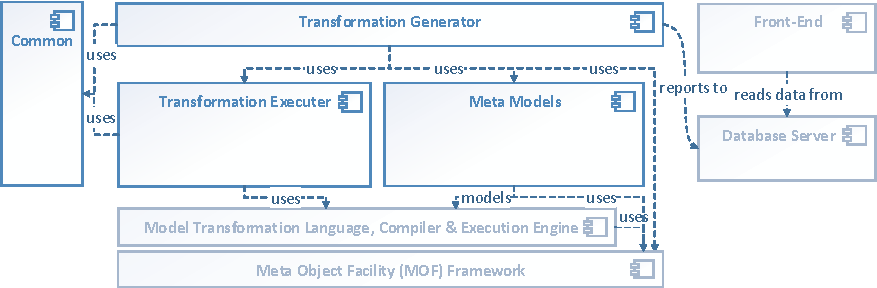
\includegraphics[scale=0.96]{Images/PrototypeArchitectureV1Overview.pdf} 
	\caption{Prototype Architecture Overview}
	\label{figPrototypeArchitectureV1Overview}
\end{figure}

The whole in-depth architecture is presented in figure \ref{figPrototypeArchitectureV1} whereas the description of the details is provided in the next sections.


\begin{landscape}
\setlength{\unitlength}{1cm}
\newsavebox{\boxPrototypeArchitectureVOne} 
\savebox{\boxPrototypeArchitectureVOne}{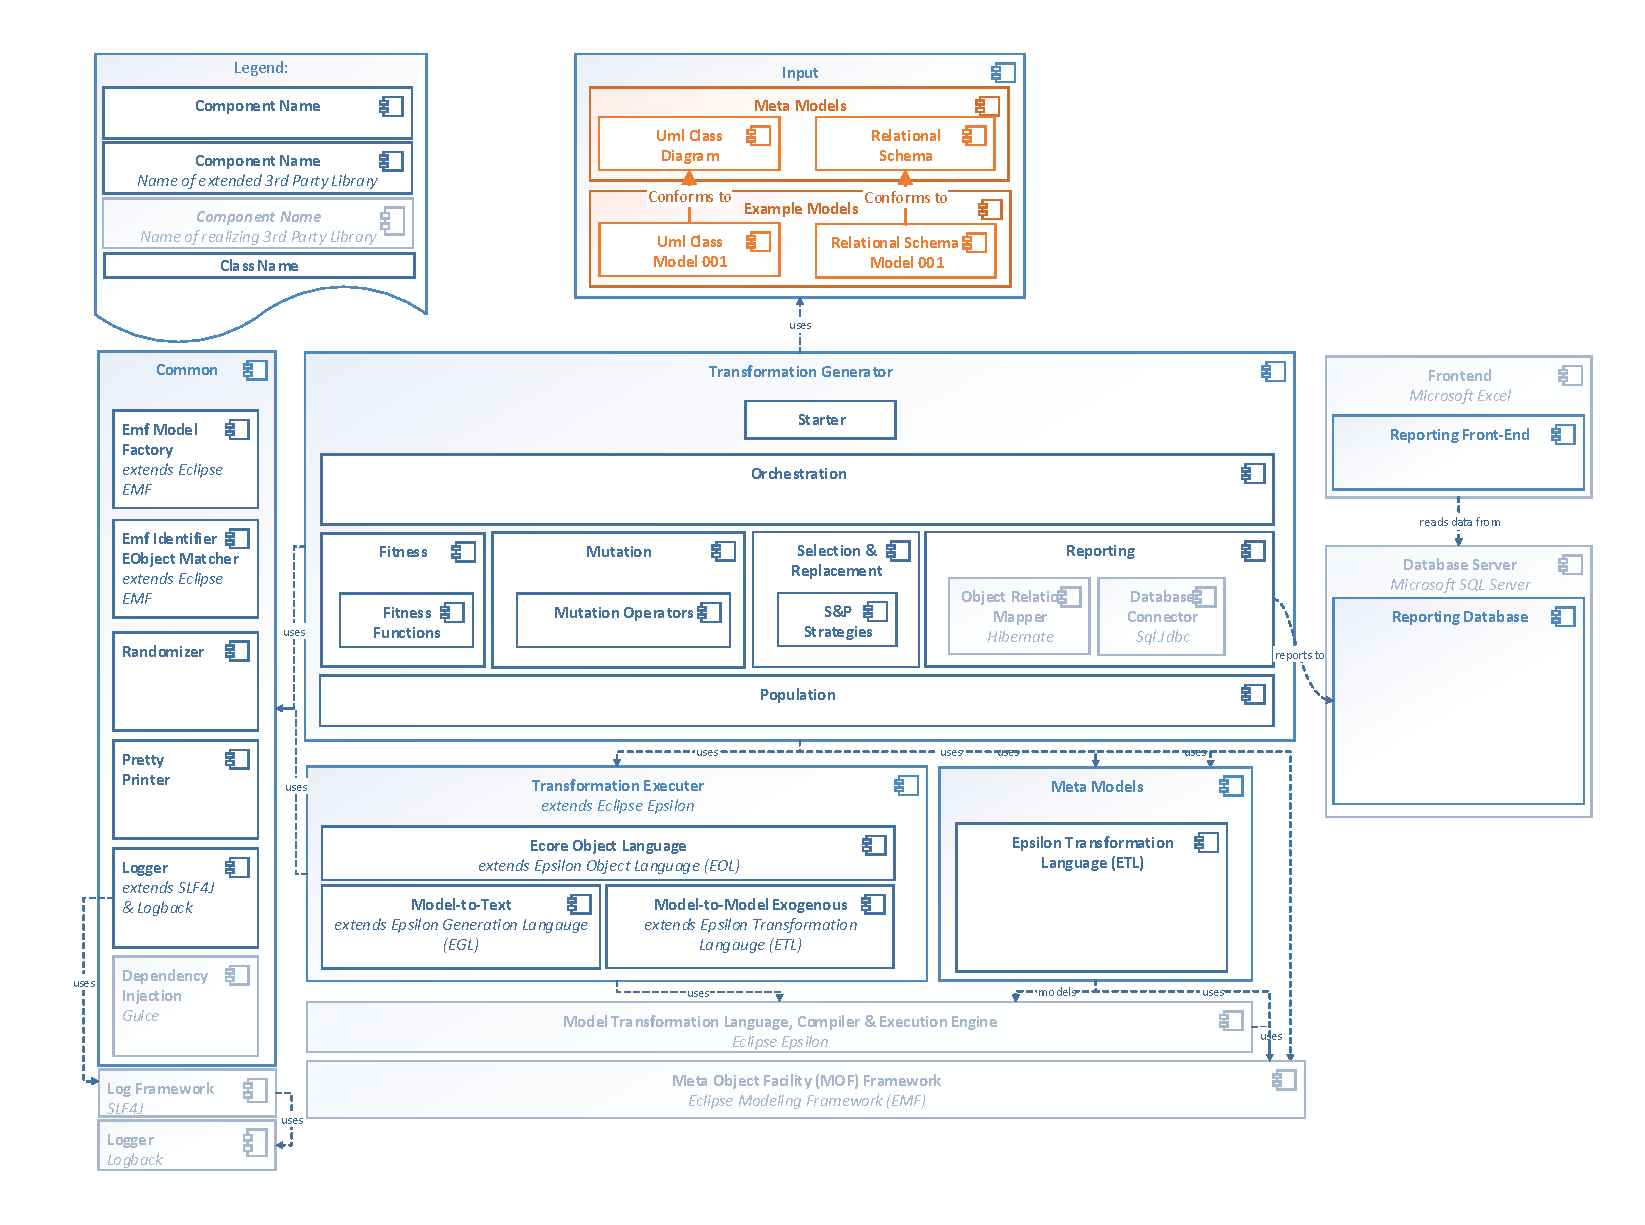
\includegraphics[scale=0.9]{Images/PrototypeArchitectureV1.pdf}} 
 \begin{figure}
   \begin{picture}(0,16.5) %-x+
  	\put(-2,0){\usebox{\boxPrototypeArchitectureVOne}} %-y+
   \end{picture} 
   \caption{Prototype Architecture}
   \label{figPrototypeArchitectureV1}  
 \end{figure}
\end{landscape}


\section{Transformation Generator}\label{secTransformationGenerator}

In order to orchestrate all the internal and external components by realizing the \gls{EvolutionaryAlgorithm}, the `Transformation Generator" is required. The main purpose is the execution of the evolution with the goal to identify a \gls{ModelToModelTransformation} for the given input \glspl{MetaModel} MM$_a$ and MM$_b$ based on the M$_a$-M$_b$ example pairs.

\subsection{Shared Data Model}
\label{secSharedDataModel}

Since the evolutionary process consists of several phases, a shared ``Population" data model is used to manage the data. This is presented in figure \ref{figPrototypeArchitectureV1PopulationDataModel}.

\begin{figure}[htb]
	\centering
	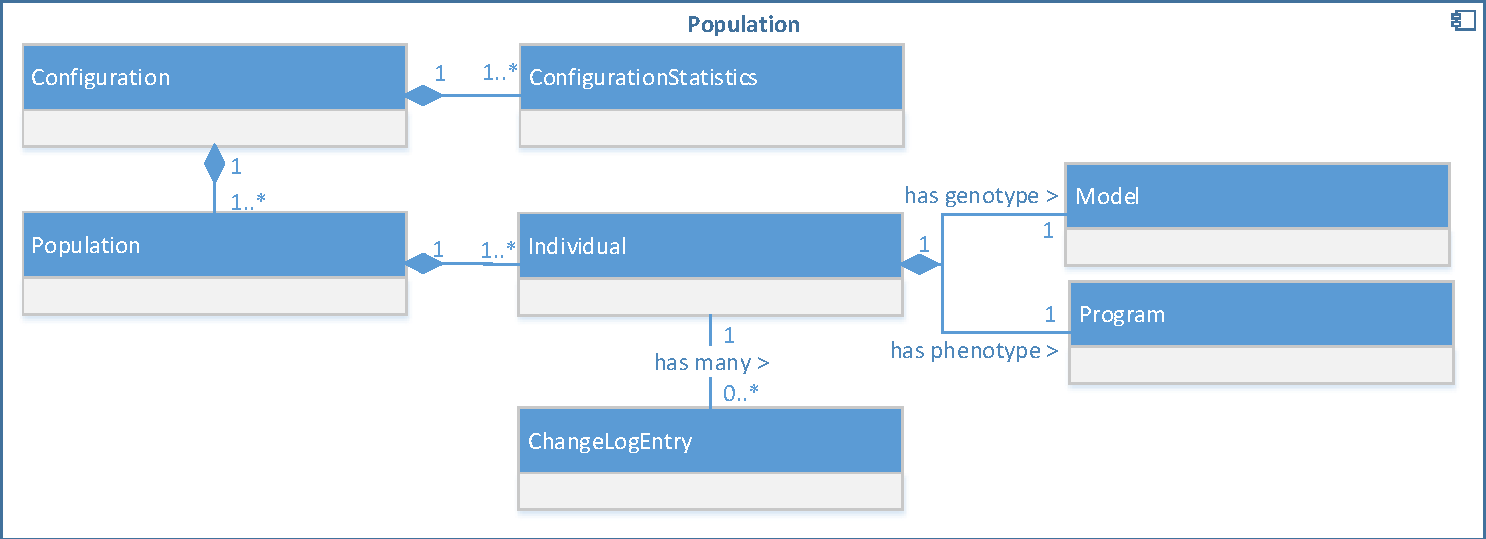
\includegraphics[scale=0.6]{Images/PrototypeArchitectureV1PopulationDataModel.pdf} 
	\caption{Prototype Population Data Model Overview}
	\label{figPrototypeArchitectureV1PopulationDataModel}
\end{figure}

%A configuration defines the settings like the \gls{FitnessFunction}, with which a \gls{Population} has been created. A \gls{Population} has the attributes ``CreatedAt" and ``CompletedAt". It consists of \glspl{Individual}, which have the attributes ``Fitness" and ``\gls{Generation}".

Based on the algorithm design in section \ref{secAlgorithmOverview}, the general structure is as follows: A \gls{Population} consists of \glspl{Individual}. Each \gls{Individual} has a ``Model" as \gls{Genotype} and a ``Program" as \gls{Phenotype}. The former contains the transformation in \gls{AbstractSyntax}, while the latter is in \gls{ConcreteSyntax}.

Since a \gls{Population} can be executed with different scenarios, \glspl{FitnessFunction}, \glspl{Mutation}, \glspl{SelectionStrategy} and \glspl{ReplacementStrategy}, all this information is stored in the ``Configuration". Additionally, there are ``ConfigurationStatistics" which contain aggregated fitness and runtime values required in the evaluation (see chapter \ref{chapEvaluation}).

With this data model the different aspects of the \gls{EvolutionaryAlgorithm} are realized in the components ``Orchestration", ``Fitness", ``Mutation" and ``Selection \& Replacement". Also, the ``Reporting" component is based on this model (see section \ref{secFrontendAndDatabaseServer}).

\subsection{Realization of Mutations}
\label{secRealizationOfMutations}

The \glspl{Mutation} are defined in section \ref{secPatternAndMutations} as a mechanism to add, remove or change a \glspl{ModelToModelTransformation} according to a pattern. In order to realize such a \gls{Mutation}, at first the \gls{Encoding} of \glspl{ModelToModelTransformation} has to be defined. There are several possibilities which are presented in the following, whereas the implemented approach is the last one:

\begin{itemize}
	\item \textbf{Simple approach based on \gls{ConcreteSyntax}}: Realize \glspl{Mutation} based on the representation of a \gls{ModelToModelTransformation} used by humans. This possibility does not provide any semantic information, which renders analysis and modifications difficult. 
	\item \textbf{Approach based on \gls{Grammar} and parse tree}: Perform a structural analysis of the transformation using its own \gls{Grammar}. Since this option still lacks precise semantic details, it is not sufficient. 
	\item \textbf{Approach based on the \gls{AbstractSyntax}}: Use the \gls{AbstractSyntax} of the \gls{TransformationExecuter}. This representation allows a precise analysis, since it is used to execute the transformation. However, it is not intended to modify the transformation. Therefore, it is designed as a super-set of the \gls{TransformationLanguage} and modifications can result in invalid transformations.
	\item \textbf{Chosen approach based on self-defined \gls{AbstractSyntax}}: In order to overcome the limitations, a new \gls{AbstractSyntax} is defined as a \gls{MetaModel}. On the one hand it enables the semantic analysis of a transformation. On the other hand it is semantically equivalent to the \gls{TransformationLanguage}. Hence, only valid modifications through \glspl{Mutation} are possible which can be designed as \glspl{ModelToModelTransformation} itself.
\end{itemize}

After providing a general overview of the realization options, the following paragraphs explain those in detail.

\textbf{Simple approach based on \gls{ConcreteSyntax}}: The first option is to implement the \glspl{Mutation} as programs that manipulate the \gls{ConcreteSyntax} of the \gls{ModelToModelTransformation}. An example for the ``One-to-One Object" add-\gls{Mutation} is a program that takes a textual representation of the transformation as an input and appends such a \gls{TransformationRule}. The drawback is that it does not scale with a large number of \glspl{Mutation}, especially in the case of sophisticated ones. Using this procedure each \gls{Mutation} needs to parse the existing transformation and add the appropriate lines of code in the right place with respect to existing constraints, which is error prone and complex.

%Therefore, the next alternatives are based on representations of the \gls{ModelToModelTransformation}, which contain semantic information. 

This representation is used to provide humans a user friendly interface, but when considering the \glspl{Mutation} there are different requirements. In general, the question is what kind of structures are allowed. For example, a \gls{TransformationRule} needs exactly one reference to a \gls{Class} of MM$_a$ and two or more to \glspl{Class} of MM$_b$. Having this knowledge, the \gls{Mutation} is able to query the kind of \glspl{Class} of MM$_a$ that are already mapped and those which are not. This is a difficult task when having only a representation like that. Without utilizing the \gls{Grammar} at all, it would result in parsing the text file. This might be a lookup for strings like ``transform", followed by an appended additional \gls{TransformationRule}. Such an append would then be a fixed string sequence, like ``rule X ...". Considering difficult expressions, which are allowed by the \gls{Grammar}, the approach is difficult to handle.

\textbf{Approach based on \gls{Grammar} and parse tree}: The next approach is to use the \gls{Grammar} to parse the existing transformation to create a parse tree representation like the one shown in figure \ref{figEtlExampleParseTree}. A simplified excerpt of this \gls{Grammar} is described in listing \ref{lstEtlGrammarFragment}, which contains two of the about 75 \glspl{ProductionRule} (see \cite{EclipseFoundation2014}) written in ANTLR 3 (\cite{Atlassian2014}). 

The first one is ``transformationRule" that defines how a \gls{TransformationRule} is structured. First, there must be the word ``rule" followed by a ``NAME" that can be any kind of string. Afterwards, there has to be a ``formalParameter" defined, which refers to a \gls{Class} of MM$_a$ and a ``formalParameterList" for one or more \glspl{Class} of MM$_b$ that are created by this \gls{TransformationRule}. Finally, a ``block" of statements has to be defined containing e.g. \gls{Property} mappings. The second \glspl{ProductionRule} is the ``formalParameter" that needs a ``NAME" and a ``typeName". The latter must refer to a \gls{Class} of MM$_a$ but that is not in scope for a \gls{Grammar}.

\begin{lstlisting}[language=ANTLR,caption={\Gls{EpsilonTransformationLanguage} specified in ANTLR \Gls{Grammar} (Simplified fragment)},label={lstEtlGrammarFragment}]
grammar EpsilonTransformationLanguage;

transformationRule
	:	'rule' NAME 
			'transform' formalParameter 
			'to' formalParameterList
			'{'
			 	block 
		'}'
	;

formalParameter
	:	NAME ':' typeName
	;
	
...
\end{lstlisting}

This allows an easier querying for existing structures, e.g. ``get all transform nodes" to analyze which \glspl{Class} of MM$_a$ have already been mapped. Since it is only used to read the transformation, not to manipulate it and write it back, this is a one-way technique. Usually, the transformation is written by humans and then parsed to be executed by the \gls{TransformationExecuter}, hence the limitation. Additionally, this representation still contains a lot of useless information in form of keywords like ``rule". This renders it difficult to mutate the parsed tree, as it on the one hand requires a lot of useless information and on the other hand is missing important information. Such an information is for example that the first ``formalParameter" must refer to a \gls{Class} of MM$_a$ or that a \gls{TransformationRule} needs exactly one ``transform" node. %The latter seems maybe not obvious as it is stated by the \gls{Grammar} but when looking at the parse tree, the information got lost as there is no direct link to the \gls{Grammar}.

\begin{figure}[htb]
	\centering
	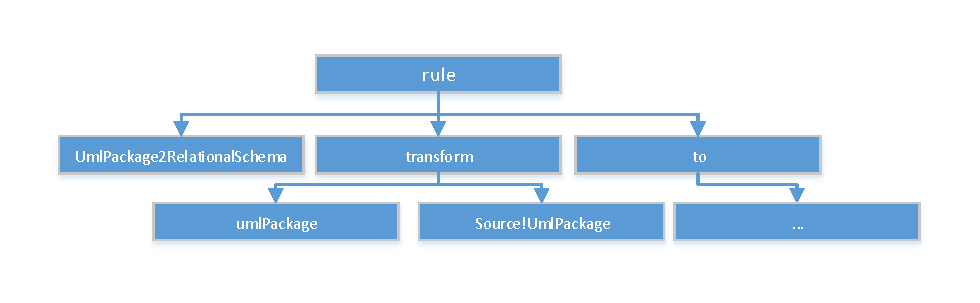
\includegraphics[scale=0.8]{Images/EtlExampleParseTree.pdf} 
	\caption{Parse tree fragment of the simple structural example}
	\label{figEtlExampleParseTree}
\end{figure}

\textbf{Approach based on the \gls{AbstractSyntax}}: The \gls{AbstractSyntax} of the chosen \gls{TransformationLanguage} \gls{EpsilonTransformationLanguage} is not explicitly provided, but could be extracted from the \gls{TransformationGenerator} (see \cite{EclipseFoundation2014}). Since it is used to execute a transformation, this \gls{AbstractSyntax} removes all aspects and constraints which are irrelevant for this task (see \cite{Bendersky2009}). The drawback is that this is a one-way approach, where the resulting language allows constructs that were not possible before due to the simplified structure. Thereby, it becomes a super-set of the \gls{EpsilonTransformationLanguage} which renders a transformation back into the \gls{ConcreteSyntax} impossible in general. This syntax could be used, if the goal of the generated transformation would only be the execution. However, the goal is to create transformations which are maintainable by humans. Hence, the resulting transformation must be provided in \gls{ConcreteSyntax}.

\textbf{Chosen approach based on self-defined \gls{AbstractSyntax}}: Since the previous approaches were not appropriate to serve as a foundation for the \glspl{Mutation}, the solution is to define an \gls{AbstractSyntax} using a \gls{MetaModel} instead, shown in figure \ref{figEtlSimplifiedFragmentOfAbstractSyntaxWithExample}. Based on the \gls{Grammar} this \gls{MetaModel} is derived manually defining an \gls{AbstractSyntax} of the \gls{EpsilonTransformationLanguage} that on the one hand excludes all keywords, but on the other hand contains the required constraints. 

The fragment in figure \ref{figEtlSimplifiedFragmentOfAbstractSyntaxWithExample} presents the idea, which is based on the listing \ref{lstEtlGrammarFragment} and figure \ref{figEtlExampleParseTree}. The \gls{MetaModel} on the left hand side specifies the structure of a ``TransformationRule" that needs exactly one ``FormalParameter" while both need a name. Whereas the instance on the right hand side is directly based on that and is enabled for queries and modifications according to the \gls{MetaModel}. Those modifications are \glspl{ModelToModelTransformation} themselves, since they are based on \glspl{MetaModel}.

\begin{figure}[htb]
	\centering
	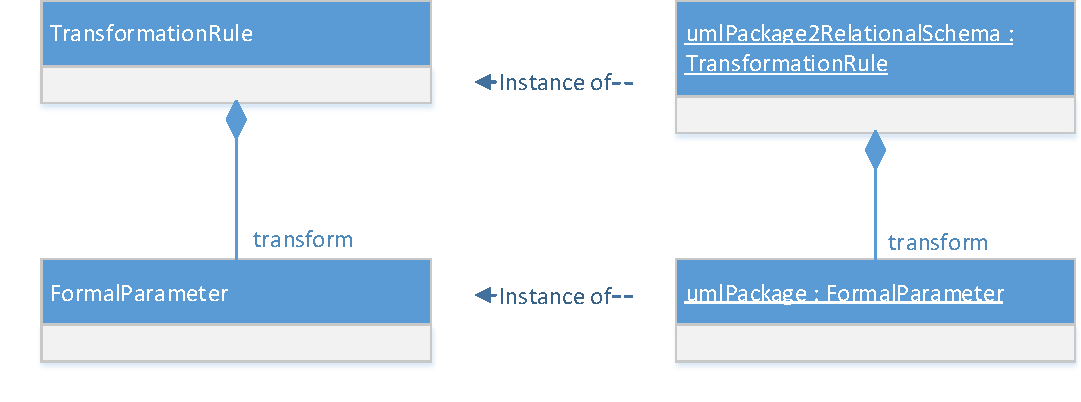
\includegraphics[scale=0.6]{Images/EtlSimplifiedFragmentOfAbstractSyntaxWithExample.pdf} 
	\caption{Simplified fragment of the \Gls{EpsilonTransformationLanguage} in \gls{AbstractSyntax} with an example}
	\label{figEtlSimplifiedFragmentOfAbstractSyntaxWithExample}
\end{figure}

This \gls{MetaModel} of the \gls{EpsilonTransformationLanguage} is insufficient, as it lacks the foundation of its input \glspl{MetaModel} MM$_a$ and MM$_b$, the \gls{MetaObjectFacility} \gls{MetaModel}. In order to create proper references also a simplified \gls{MetaObjectFacility} \gls{MetaModel}, based on the one from section \ref{secModelLanguage}, is added to the \gls{EpsilonTransformationLanguage} \gls{MetaModel}.

Figure \ref{figMofSimplifiedFragmentOfAbstractSyntaxWithExample} shows this extension. It contains a ``MofClass" with its ``MofProperties", both derived from a ``MofNamedElement" as each requires a ``Name". Additionally, ``MofProperties" can be associated with a ``MofAssociation" that includes at least two of them. In the context of the simple structural example, an instance of a ``MofClass" is a ``umlPackage" with a ``MofProperty" ``umlPackageName".

\begin{figure}[htb]
	\centering
	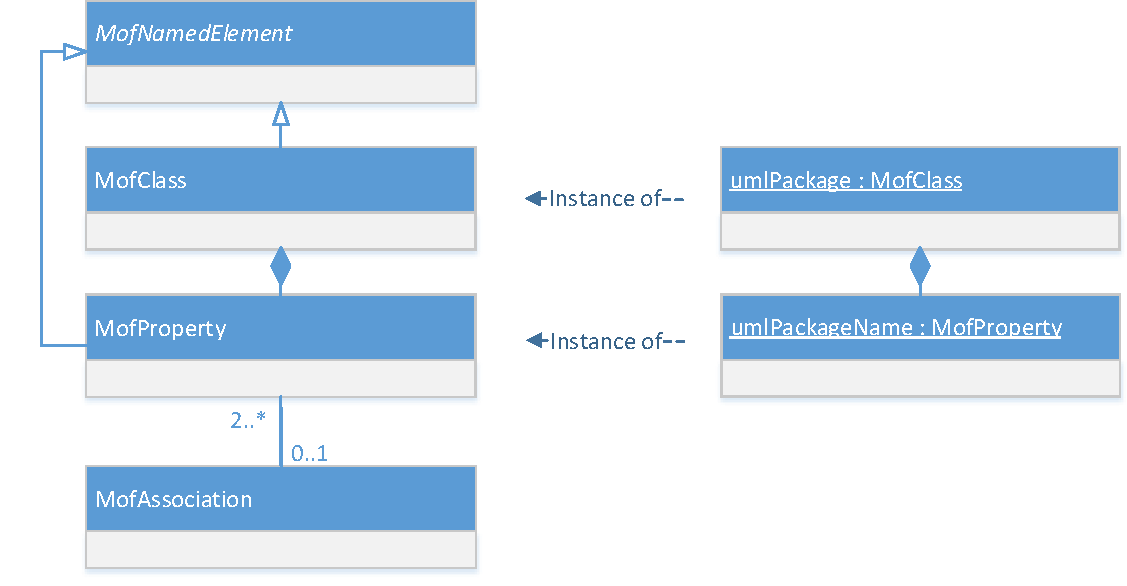
\includegraphics[scale=0.6]{Images/MofSimplifiedFragmentOfAbstractSyntaxWithExample.pdf} 
	\caption{Simplified fragment of \Gls{MetaObjectFacility} in \gls{AbstractSyntax} with an example}
	\label{figMofSimplifiedFragmentOfAbstractSyntaxWithExample}
\end{figure}

The usage of the extension is presented in figure \ref{figEtlandMofAbstractSyntaxReferenceExample}, which combines the examples from figure \ref{figEtlSimplifiedFragmentOfAbstractSyntaxWithExample} and \ref{figMofSimplifiedFragmentOfAbstractSyntaxWithExample}. As it is possible to reference to the MM$_a$ and MM$_b$ \gls{MetaModel} \glspl{Class} and \glspl{Property}, the ``umlPackage : FormalParameter" can be directly related to the ``umlPackage : MofClass".

\begin{figure}[htb]
	\centering
	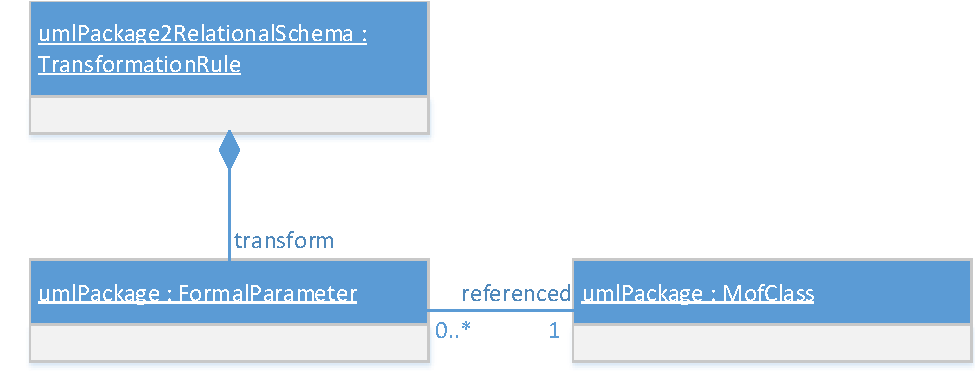
\includegraphics[scale=0.6]{Images/ETLandMofAbstractSyntaxReferenceExample.pdf} 
	\caption{Example of a reference in an instance of the \gls{AbstractSyntax} of the combined \Gls{EpsilonTransformationLanguage} and \Gls{MetaObjectFacility}}
	\label{figEtlandMofAbstractSyntaxReferenceExample}
\end{figure}

Based on this \Gls{EpsilonTransformationLanguage} and \Gls{MetaObjectFacility} \glspl{MetaModel} the \glspl{Mutation} are defined. Since this is an \gls{Endogenous} transformation, there is a \gls{DomainSpecificLanguage} also in the language framework of \gls{EpsilonTransformationLanguage}, which is the \gls{EpsilonWizardLanguage} (see \cite{Kolovos2013}). This language was replaced during the implementation phase with a self-designed, embedded transformation \gls{DomainSpecificLanguage} in Java 8. Further details about this decision are provided in the sub-section \ref{ModelToModelTransformationFramework}.

Using the \gls{Mutation} specific \gls{AbstractSyntax} instead of the \gls{ConcreteSyntax} adds the additional task of transforming the former into the latter in order to provide a result which is maintainable by humans. Additionally, it is also required to execute it with the \gls{TransformationExecuter} of the \gls{EpsilonTransformationLanguage}. This \gls{ModelToTextTransformation} is shown partially in listing \ref{lstEglModelToTextFragment}. %This task could also be solved by transforming the self-defined \gls{AbstractSyntax} into the \gls{TransformationExecuter} \gls{AbstractSyntax}. However, in this case this is an avoidable additional effort since the \gls{TransformationExecuter} uses the  

The first operation transforms an ``EtlTransformationRule" and adds the required tags defined in listing \ref{lstEtlGrammarFragment} like ``rule", ``transform" and ``to". The second operation creates the syntax required for a ``EolMofClassFormalParameter". The first operation is linked to the second one via the call of ``self.sourceParameter" and the second one for the target. According to the \gls{MetaModel} an ``EtlTransformationRule" has a ``sourceParamter" \gls{Property} of type ``EolMofClassFormalParameter". Hence, the second operation is invoked with the required parameter ``prefix" through the appended method call ``.toText('Source')". The statically provided ``Source" and ``Target" strings are used as a convention to refer to MM$_a$ and MM$_b$.

\begin{lstlisting}[language=EGL,caption={\Gls{ModelToTextTransformation} of the \gls{AbstractSyntax} (\Gls{EpsilonTransformationLanguage} \gls{MetaModel}) into the \gls{ConcreteSyntax} (\Gls{EpsilonTransformationLanguage} \gls{Grammar}) specified in the \Gls{EpsilonGenerationLanguage} (Simplified fragment)},label={lstEglModelToTextFragment}]
@template
operation EtlTransformationRule toText() { 	
%]
	rule [%= self.name %]
		transform [%= self.sourceParameter.toText("Source") %]
		to	  [%= self.targetParameters
										.collect( tp | tp.toText("Target") )
										.concat(",") %] {
		[% if (self.body.isDefined()) { %]
			[%= self.body.toText() %]
		[% } %]
	}
[%
} 

@template
operation EolMofClassFormalParameter toText(prefix) { 
	%][%= self.name %] : [%= prefix %]![%= self.referenced.name %][%
}
\end{lstlisting}

\subsection{Mutation and Fitness Evaluation Process}
\label{secMutationProcess}

After providing an overview of the general realization of the \glspl{Mutation}, the mutation and fitness evaluation process presented in figure \ref{figMutationOperatorDesign} is described.

As previously described, the approach is to convert the given entities from \gls{ConcreteSyntax} into the \gls{AbstractSyntax}, which is the foundation to apply \glspl{ModelToModelTransformation}. Therefore, the \gls{TransformationLanguage} \gls{Grammar} of the \gls{EpsilonTransformationLanguage} (\cite{EclipseFoundation2014}) and parts of \gls{MetaObjectFacility} have been translated into the \gls{TransformationLanguage} \gls{MetaModel} and a simplified \gls{MetaObjectFacility} \gls{MetaModel} (see figure \ref{figEtlSimplifiedFragmentOfAbstractSyntaxWithExample}) once.

Applying this foundation to a transformation scenario where a ``MM$_a$ $\rightarrow$ MM$_b$ Transformation" has to be created (see listing \ref{lstETLSimpleExample} for a simple structural example), there must be the \glspl{MetaModel} MM$_a$ and MM$_b$ provided in \gls{ConcreteSyntax} (MM$_a$ example see figure \ref{figScenarioStructuralSimpleUmlClassMetaModel}, MM$_b$ example see figure \ref{figScenarioStructuralSimpleRelationalMetaModel}). 

Based on those there have to be one or more M$_a$-M$_b$ pairs provided that are instances of MM$_a$, MM$_b$ respectively, and are semantically identical (M$_a$ example see figure \ref{figScenarioStructuralSimpleUmlClassModel1}, M$_b$ example see figure \ref{figScenarioStructuralSimpleRelationalModel1}).

In order to begin the mutation process for such a scenario, at first the \glspl{MetaModel} MM$_a$ and MM$_b$ must be converted into the \gls{AbstractSyntax} based on the simplified \gls{MetaObjectFacility} \gls{MetaModel} (see figure \ref{figMofSimplifiedFragmentOfAbstractSyntaxWithExample}). Those \glspl{MetaModel} are referred from the ``MM$_a$ $\rightarrow$ MM$_b$ Transformation" in the \gls{AbstractSyntax} (see figure \ref{figEtlandMofAbstractSyntaxReferenceExample}).

The transformation, which is an empty one at the beginning, is then created or modified by applying the previously defined \glspl{Mutation} executed by the \gls{TransformationGenerator}. Afterwards, this ``MM$_a$ $\rightarrow$ MM$_b$ Transformation" in \gls{AbstractSyntax} has to be translated into \gls{ConcreteSyntax} in order to be executable (see figure \ref{lstEglModelToTextFragment}).

Finally, the \gls{TransformationExecuter} executes the transformation with each given M$_a$ of the example pairs and outputs a M$_b$ \gls{Model} as well as the \glspl{Trace}. The created M$_b$ \glspl{Model} are then compared with the expected M$_b$ \glspl{Model} from the example pairs resulting in a fitness of each pair.

%Applying this process to the simple structural example defined in section \ref{lstETLSimpleExample} results in the following steps.

\begin{landscape}
\setlength{\unitlength}{1cm}
\newsavebox{\boxMutationOperatorDesign} 
\savebox{\boxMutationOperatorDesign}{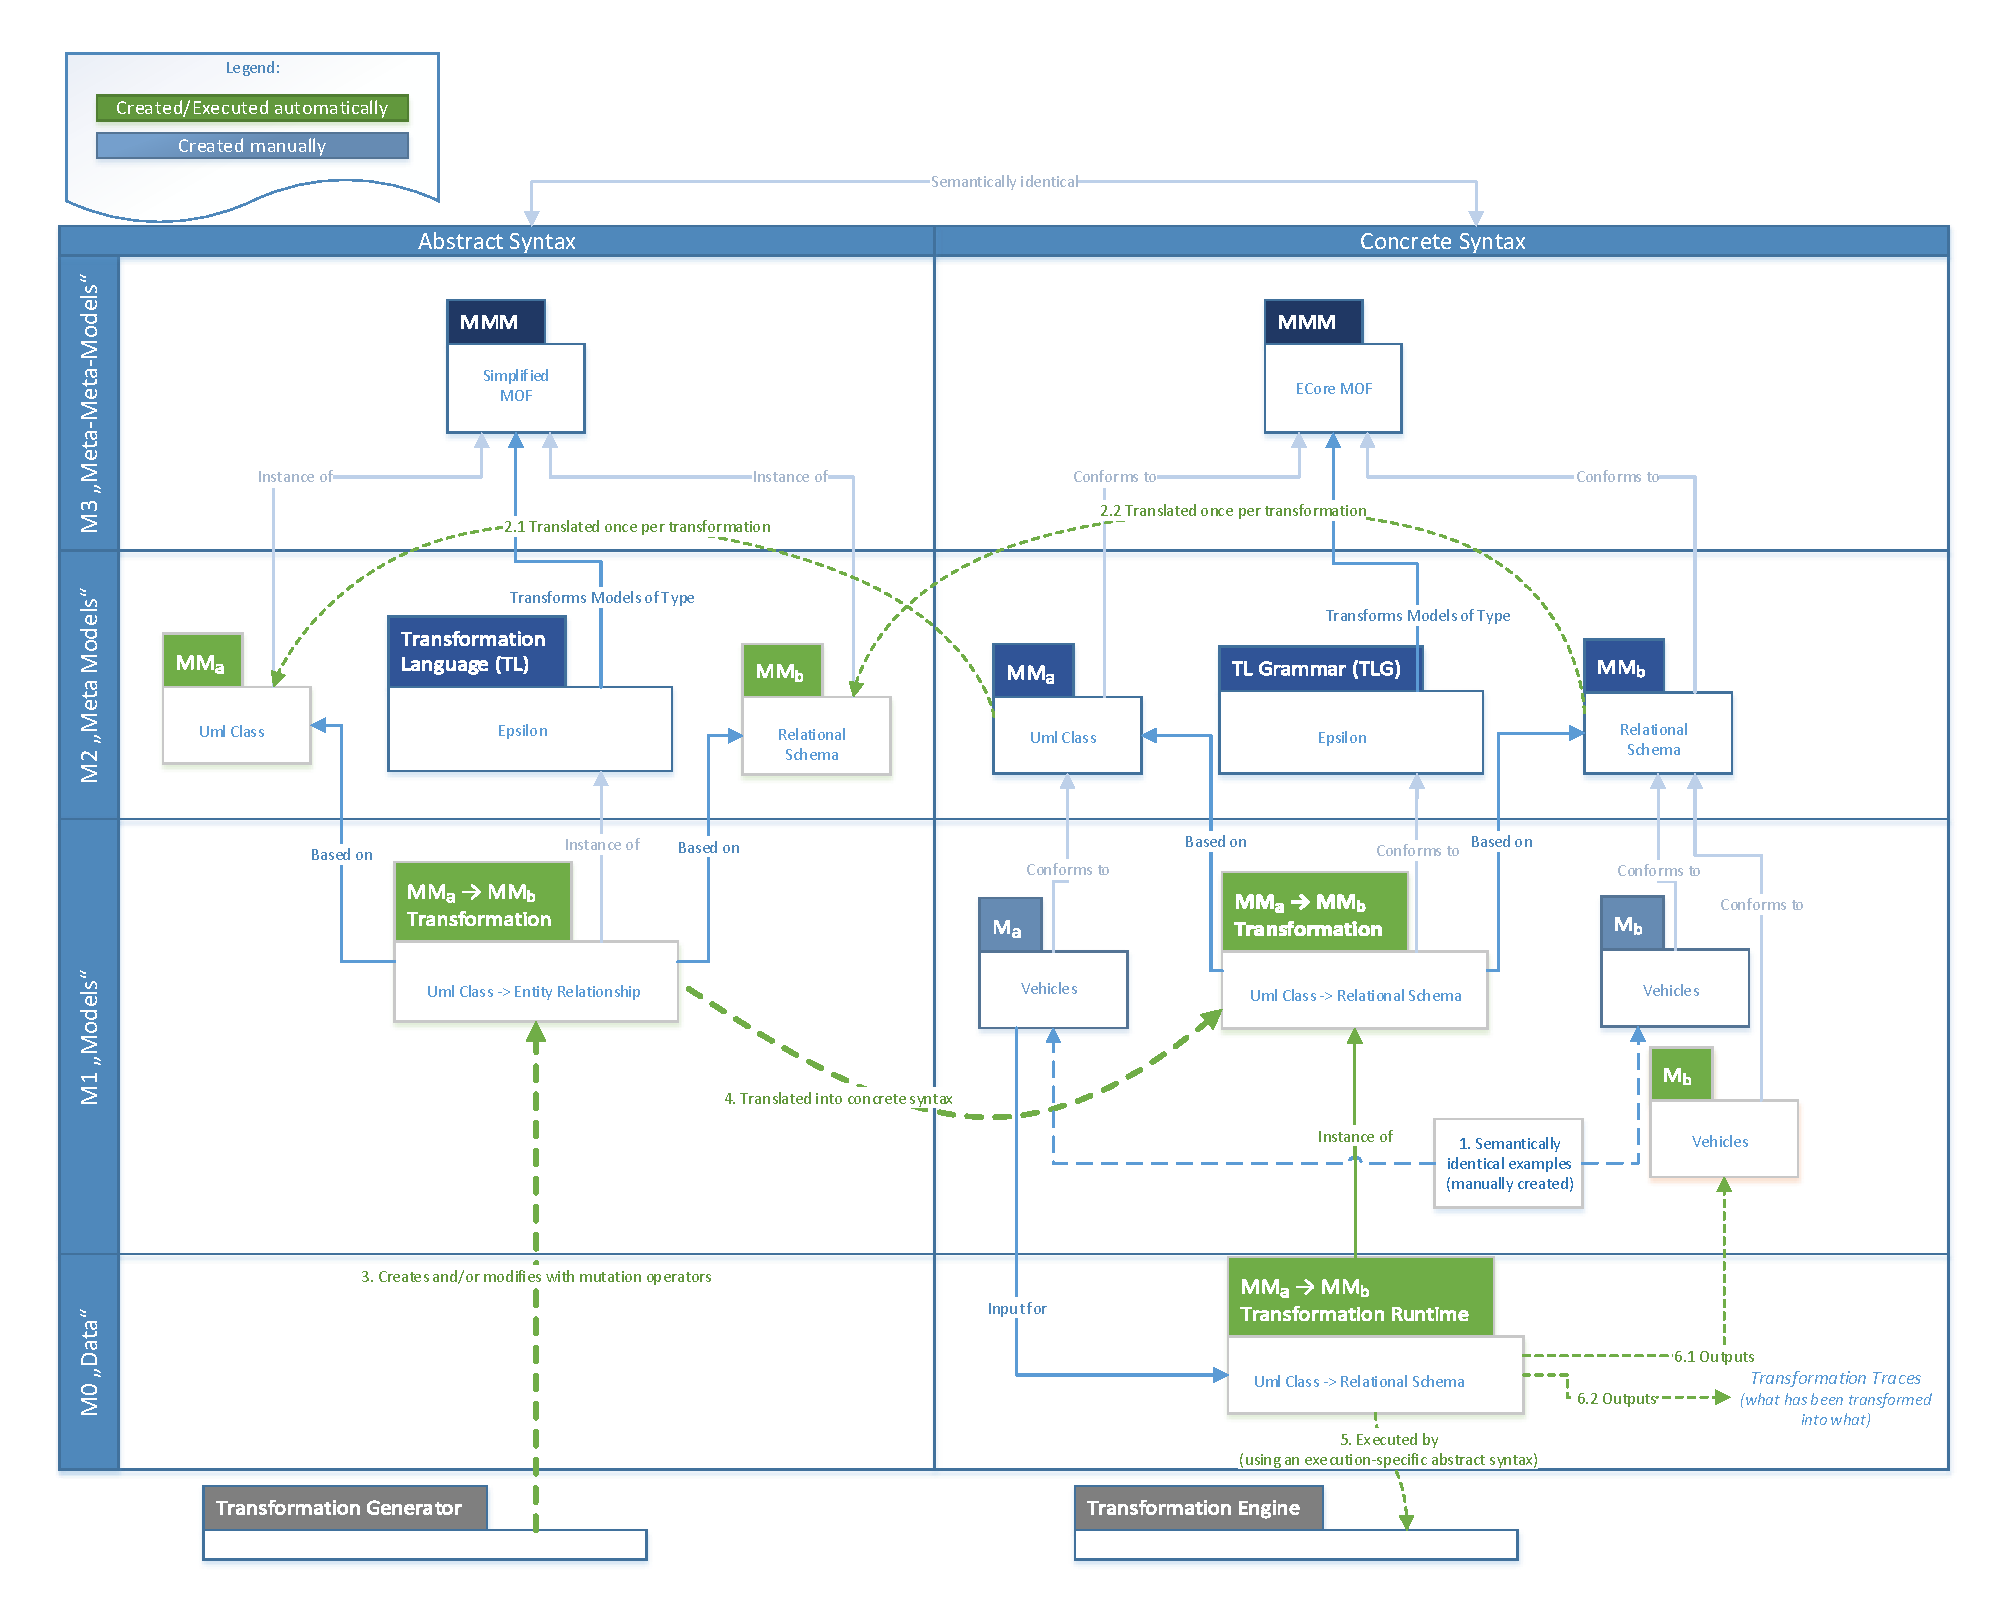
\includegraphics[scale=0.72]{Images/MutationOperatorDesign.pdf}} 
 \begin{figure}
   \begin{picture}(0,16.5) %-x+
  	\put(-2,0){\usebox{\boxMutationOperatorDesign}} %-y+
   \end{picture} 
   \caption{Mutation and Fitness Evaluation Process Overview}
   \label{figMutationOperatorDesign}  
 \end{figure}
\end{landscape}


%TODO change secTransformationsAndMetaModels
%As designed in section \ref{secPatternAndMutations} and also described in \ref{secMetaModels}, the ``Mutation" component does not only contain a basic execution stub for the \gls{Mutation} transformation execution. It also contains a component for each transformation that creates instances for all possible combinations of input parameters.

% - algorithm process: algorithmic framework vs self impl
	% -> KEY QUESTION: mutation operators: OO, M2M transformations ??
	% -> explain tricky parts and general concept (based on refined problem domain)
		% -> explain with examples (abstract syntax, grammar etc...)
	% -> introduce generator, engine
	% --> technological choices for both... explain decision 
	
% - prototype architecture
	% ...
	% -> reporting example

\section{Third Party Frameworks}\label{secThirdPartyFrameworks}

In this section the selection of third party frameworks is explained. In particular, it includes the definition of requirements. Furthermore, the proportionality of the provided features on the one hand and the introduced constraints on the other hand must overall result in a reduced effort.

Based on chapter \ref{chapAlogrithmDesign} the following areas have been identified for the application of external frameworks: The \gls{EvolutionaryAlgorithm} itself might be supported by a framework, the various \glspl{ModelToModelTransformation} and the evaluation of the algorithm. Additionally, the maintainability and testability of the whole application can be improved by a dependency injection framework.

\subsection{Evolutionary Algorithm Framework}
\label{subsecEvolutionaryAlgorithmFramework}
The most important question is how to realize the \gls{EvolutionaryAlgorithm} itself, since this decision has an impact on all the other components. On the one hand, there are several existing \gls{GeneticAlgorithm} frameworks, but only a few for this specific task called ``Strongly Typed Genetic Programming Algorithm" (see \cite{Montana2002}). This part of the discipline is one of the most challenging tasks, since the \glspl{Mutation} need to respect non-trivial constraints. For example, the definition of a variable has to occur before the usage, or a return type of a function must be compatible in the case the function is changed.

Since the approach is based on a \gls{MetaModel}, with \glspl{Mutation} being \gls{Endogenous} \glspl{ModelToModelTransformation}, none of the existing frameworks is able to handle this task (\cite{McDermott}, \cite{Meffert}, \cite{Lukasiewycz}). The fundamental \gls{GeneticProgramming} algorithm entities are rather simple, hence adapting an existing framework is not appropriate. Thus, no framework is used. % is only appropriate, if it is intended for this simple approach. %Therefore, the \gls{EvolutionaryAlgorithm} is implemented without any third party frameworks.

\subsection{Model-to-Model Transformation Framework}
\label{ModelToModelTransformationFramework}

The requirements for a \gls{ModelToModelTransformation} framework are defined in sub-section \ref{secExistingModelTransformationLanguagesAndTools}. Also, the existing languages are presented and the \gls{TransformationLanguage} \gls{EpsilonTransformationLanguage} (\cite{Kolovos2013}) is chosen. Since the Eclipse Epsilon programming interface is implemented in Java (\cite{Oracle}), this language is used as the programming language for the whole solution.

Within the realization design of \glspl{Mutation} in sub-section \ref{secRealizationOfMutations}, the \gls{EpsilonGenerationLanguage} is used for the \gls{ModelToTextTransformation}. It is also part of the Epsilon framework. \Gls{Exogenous} \glspl{ModelToModelTransformation} inside the \glspl{Mutation} are implemented using Java 8. The new language features, especially lambda functions, enable Java as a \gls{TransformationLanguage} with similar language features as the transformation \glspl{DomainSpecificLanguage} (\cite{Rachev2012}). Together with the existing Java features and tool-set, the implementation and testing capabilities are superior compared to \glspl{DomainSpecificLanguage} like the \gls{EpsilonTransformationLanguage}. This language is therefore chosen as the host for the self-designed, embedded transformation \glspl{DomainSpecificLanguage}. %Nevertheless Java is not a \glspl{DomainSpecificLanguage}, hence it does not provide any specific guidelines or restrictions.

As already mentioned in section \ref{secModelLanguage}, a \gls{TransformationLanguage} needs also a language as a foundation for the \glspl{MetaModel} MM$_a$ and MM$_b$. In general, the \gls{MetaObjectFacility} is chosen, but nevertheless an implementation is required that is compatible with Eclipse Epsilon, which is the \gls{EclipseModelingFramework} (\cite{EMF}). It provides a large set of utilities e.g. to read and write models. 

Since the decision for the \gls{EclipseModelingFramework} is directly related to the decision for the \gls{EpsilonTransformationLanguage}, no alternatives are considered.

The \gls{TransformationLanguage} is targeted at file based, single user applications. This is a disadvantage considering the requirement to create and use \glspl{Model} and their \glspl{MetaModel} in an \gls{EvolutionaryAlgorithm}, where each \gls{Individual} is independent from the others. In the case all model related operations are file based and cannot be executed in parallel, this causes a bottleneck. Therefore, the extension ``Emf Model Factory" has been implemented which is presented in section \ref{secCommon}.

\subsection{Reporting Framework and Logging Framework}\label{subsecReportingFrameworkAndLoggingFramework}

To analyze the \gls{EvolutionaryAlgorithm} the development of the \glspl{Individual} and the whole \gls{Population} has to be tracked. In the integration test phase, this is the most important use case, in order to determine the root cause for non-termination.

The solution is twofold: First, the fitness and the \gls{Generation} of each \gls{Individual} is stored in a relational database. Thereby existing analysis tools for large datasets could be used to track the hundreds or thousands of \glspl{Individual} down to the ones which are relevant for a further analysis or to aggregate them, to inspect the algorithm performance. Second, the in depth analysis of the evolution of an \gls{Individual} can be analyzed with the logging framework.

As a database engine Microsoft SQL Server 2012 (\cite{Microsoft}) is used and the analysis tool is Microsoft Excel 2013 (\cite{Microsofta}). The combination of both avoids the time consuming implementation of an own analysis front-end. Furthermore, an interface from the object-oriented programming language Java to the relational database is required, which is the similarly well established Hibernate (\cite{JBossCommunity}) Object-Relational-Mapper (ORM).

The logging framework chosen consists of the actual logger Logback (\cite{QualityOpenSoftwarea}) and a generic logging interface SLF4J (\cite{QualityOpenSoftware}). The latter ensures that in case of changing requirements the actual logger could be easily exchanged.

\subsection{Dependency Injection}

A common pattern to separate functionality and interfaces is dependency injection (\cite{Knauß}). As the whole solution uses a lot of external functionality, it is necessary for unit tests to use mocks, or also called dummies, instead of the actual implementation. Mocks are test-specific implementations of an interface in order to keep the unit-test focused only on the relevant components. Having dependency injection in place, a component can be easily replaced.
 
In the case an internal or external component needs to be exchanged by another implementation,  which is likely, this is much easier when using dependency injection.

The overhead of using dependency injection is rather small, which results overall in a reduced effort.

The selected framework for dependency injection is Guice (\cite{Google}).

\section{Meta Models}\label{secMetaModels}

The \glspl{MetaModel} component contains the definition of \gls{MetaObjectFacility} and \gls{EpsilonTransformationLanguage} (see figure \ref{figEtlSimplifiedFragmentOfAbstractSyntaxWithExample}).

\section{Transformation Executer}\label{secTransformationExecuter}

The Epsilon framework is designed for single users developing and executing transformations based on files. Hence, the implementation is also heavily tied to the Eclipse user interface.

Since the \gls{EvolutionaryAlgorithm} handles hundreds or thousands of \glspl{Individual}, each mutating on its own, there is a need for parallel and fast processing. Both cannot be implemented by using the Epsilon framework directly. 

Therefore, the ``Transformation Executer" component primarily provides a programming interface that can be used without a user interface. Furthermore, it removes the need for file based operations and replaces it with in-memory operations. 

Since Epsilon is based on the \gls{EclipseModelingFramework}, which was designed with similar user-focused requirements, also the ``Emf Model Factory" component is necessary (see sub-section \ref{subsecEmfModelFactory}).

\section{Reporting Front-end and Database Server}\label{secFrontendAndDatabaseServer}

In order to store the information about the evolution of \glspl{Individual} and the \gls{Population}, a relational database is used (see sub-section \ref{subsecReportingFrameworkAndLoggingFramework}). 

The database schema contains the tables ``Configuration", ``ConfigurationStatistics", ``Population" and ``Indivdual" (see section \ref{secTransformationGenerator}). With this data structure the relevant measurement values are stored and used among different aggregated analysis reports in the excel front-end (see chapter \ref{chapEvaluation}). Additionally, the database contains views and stored procedures. They are required to pre-process the data for the front-end.

Within the Excel-based front-end an analysis of all finished executions is possible. The analysis is based on the configuration options. Examples of the resulting charts are presented in chapter \ref{chapEvaluation}.

%Based on this information in the relational database, the excel front-end has been set-up.

% The primary report has two axis (see \ref{figExcelReportingFrontend}). On the x-axis there is the \gls{Generation} and on the y-axis is the maximum, average and minimum fitness aggregated over all \glspl{Individual} of a \gls{Generation}.

%From a algorithmic point of view the latter might also be stored per \gls{Population}, but from an implementation perspective it is more extensible 

\section{Common}\label{secCommon}

All re-usable, generic functionality that is required by the ``\Gls{TransformationGenerator}" and the ``\Gls{TransformationExecuter}" is located in this component.

\subsection{Emf Model Factory}\label{subsecEmfModelFactory}
Among the Common-components, the most important one is the ``Emf Model Factory". As already described in section \ref{secTransformationExecuter}, the \gls{EclipseModelingFramework} has been designed for single user, file-based operations, but required are parallel, in-memory operations.

Hence, this component has to provide the missing capability to load, modify and clone models in a multi-threaded environment without avoidable file operations.

\subsection{Emf Identifier EObject Matcher}

This \gls{EclipseModelingFramework} extension is required for some of the \glspl{FitnessFunction} in order to compare \glspl{Object} of M$_a$ and M$_b$. In the default implementation the comparison is implemented in two steps. The first one is a comparison based on an identity \gls{Property}, in this case the ``Name" of the \glspl{Object}. If the defined \gls{Property} cannot be found or the \gls{Property} has no value, the fall-back mechanism is used. This is a heuristic that compares the \glspl{Object} based on their general \glspl{Property} and \glspl{Association} equivalence. Since all example \glspl{Model} have a ``Name"-\gls{Property}, the fall-back is only used in rare cases. Thus, the extension is required, which uses the heuristic method in the case there was no match in the first step.

\subsection{Randomizer}

Since \glspl{Mutation}, \glspl{SelectionStrategy} and \glspl{ReplacementStrategy} require randomly selected numbers of a given interval, this component must provide functions to create random numbers or randomize enumerations.

\subsection{Pretty Printer}

The \glspl{Model} which are used, especially the \gls{MetaModel} of the \gls{EpsilonTransformationLanguage}, are often large. Therefore, the ``Pretty Printer" has to flatten those structures to a simple, readable string. This is especially used to track down issues and to analyze the result of \glspl{Mutation}.

\subsection{Logger}

This component is used to extend the external logging framework described in section \ref{subsecReportingFrameworkAndLoggingFramework}. It contains extensions which are required to standardize log messages.
